\documentclass[11pt,a4paper,english]{article}
\usepackage[english]{babel} % Using babel for hyphenation
\usepackage{lmodern} % Changing the font
\usepackage[utf8]{inputenc}
\usepackage[T1]{fontenc}

\usepackage[colorlinks=true]{hyperref}

%\usepackage[moderate]{savetrees} % [subtle/moderate/extreme] really compact writing
\usepackage{tcolorbox}
\tcbuselibrary{hooks}
\usepackage[parfill]{parskip} % Removes indents
\usepackage{amsmath} % Environment, symbols etc...
\usepackage{amssymb}
\usepackage{float} % Fixing figure locations
\usepackage{multirow} % For nice tables
%\usepackage{wasysym} % Astrological symbols
\usepackage{graphicx} % For pictures etc...
\usepackage{enumitem} % Points/lists
\usepackage{physics} % Typesetting of mathematical physics examples: 
                     % \bra{}, \ket{}, expval{}
\usepackage{url}

\definecolor{red}{RGB}{255,10,10}

% To include code(-snippets) with æøå
\usepackage{listings}
\lstset{
language=c++,
showspaces=false,
showstringspaces=false,
frame=l,
}

\tolerance = 5000 % Bedre tekst
\hbadness = \tolerance
\pretolerance = 2000

\numberwithin{equation}{section}

\newcommand{\conj}[1]{#1^*}
\newcommand{\ve}[1]{\mathbf{#1}} % Vektorer i bold
\let\oldhat\hat
\renewcommand{\hat}[1]{\oldhat{#1}}
\newcommand{\trans}[1]{#1^\top}
\newcommand{\herm}[1]{#1^\dagger}

\newcommand{\Real}{\mathbb{R}}
\newcommand{\bigO}[1]{\mathcal{O}\left( #1 \right)}

\newcommand{\di}{\mathrm{d}}
\newcommand{\magM}{\mathcal{M}}

\newcounter{algcounter}
\renewcommand{\thealgcounter}{\Roman{algcounter}}

\newenvironment{algorithm}{%
\refstepcounter{algcounter}
\begin{tcolorbox}
\centerline{Algorithm \thealgcounter}\vspace{2mm}
}
{\end{tcolorbox}}

\newcommand{\figurewidth}{.85\textwidth}

\title{FYS3150/4150\\Computational Physics\\Project 4}
\author{Magnus Ulimoen (33) \& Krister Stræte Karlsen (63)}
\date{\today}

\begin{document}
\tcbset{before app=\parfillskip0pt}
\maketitle

\begin{abstract}
This project explores the Ising model applied to spins in two dimensions.
The critical temperature for the Ising model is determined and some
parameters are calculated.
\end{abstract}



\section{Introduction}

The Ising model is a simple model of a solid. A lattice with elements 
each have a spin. This interaction between the different spin states
give an energy. The net amount of spin in the 
lattice leads to an overall magnetisation. 

Which energy the lattice 
is permitted to have is controlled by a large heat reservoir. If 
the temperature is large, the spins tends to be randomly aligned, 
and there is no net magnetisation. The highest temperature which 
allows a magnetisation is called the Curie temperature, and is 
connected to a phase transition.

The programs belonging to this report is available at 
\url{https://github.com/mulimoen/FYS3150CompPhy} under Project 4.

\section{Theory}

The energy of a spin system in the Ising model is given by
\begin{gather}
E = -J\sum_{\expval{kl}}^N s_k s_l
\end{gather}
Here J is the energy shared between two lattice points. $s_i$ is the spin
connected to the lattice point. This spin has a value of $\pm 1$.

The summation $\expval{kl}$ only sums over pairwise interactions.
Another way of writing the sum is to only consider the forward 
interaction between the lattice points,
\begin{gather}
E = -J \sum_{k}^N s_k s_{k+1}
\label{eq:Esum}
\end{gather}
This sum faces a boundary problem. In our model we are solving this 
by using periodic boundary conditions,
\begin{gather}
s_k = s_{k \pm L}
\label{eq:boundary}
\end{gather}
An illustration of this is visible in figure \ref{fig:spin_neighbours_full}.
Here the spin $S_2$ faces $S_4$ both on the upper and lower site.

\begin{figure}[H]
\centering
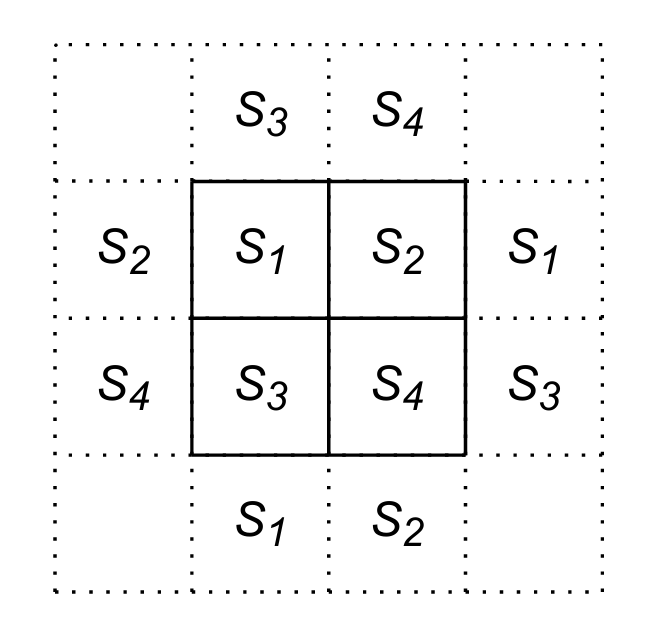
\includegraphics[scale=0.15]{pics/pics4report/simple_lattice.png}
\caption{ Illustration of the simple, ''$L=2$''-lattice and a graphical interpretation the periodic boundary conditions.}
\label{fig:spin_neighbours_full}
\end{figure}

The magnetisation of the lattice is given by the sum of the elements,
\begin{gather}
\magM = \sum_i s_i
\label{eq:Msum}
\end{gather}


\subsection{Statistical mechanics}
In order to find how the energy and magnetisation is in the steady-state
solution some results from statistical mechanics is employed. These 
give expectation values in the thermodynamic limit, which is the limit 
where the number of samplings and particles goes to infinity.

The steady-state solution has a close connection to the temperature 
of the system. If our system is connected to a heat reservoir, we can
give the probability by the Boltzmann probability function,
where he probability to find the system in a microstate is given by
\begin{gather}
p(i) = \frac{e^{-E_i\beta}}{Z}
\end{gather}
Where $E_i$ is the energy for the microstate, $\beta = \frac{1}{kT}$ 
and Z is the partition function. The partition function works as the 
normalisation factor, and is given by
\begin{gather}
Z = \sum_i \exp(-\beta E_i)
\end{gather}

\subsubsection{Energy}
The energy of the system can be calculated from the partition function
by the equation
\begin{gather}
\expval{E} = -\frac{d \ln Z}{d \beta}
\end{gather}
One useful quantity is the heat capacity, how much energy the system 
retains when changing the temperature. This quantity is given by
\begin{gather}
C_v = \frac{d\expval{E}}{dT} 
= -\frac{\beta^2}{k}\frac{d\expval{E}}{d\beta}
 = \frac{\beta^2}{k}\frac{d^2\ln Z}{d^2\beta}
\end{gather}



\subsubsection{Magnetisation}
From the partition function the magnetisation can be found. If all the 
states with a certain magnetisation is known, 
\begin{gather}
\expval{\magM} = \sum_i m_i p(m_i) = \sum_i \frac{M_i e^{-E_i\beta}}{Z}
\end{gather}
Another important quantity is the susceptibility. This is how much 
magnetisation is reatained when the temperature changes,
\begin{gather}
\chi = \frac{d \expval{\magM}}{d T} 
= -\frac{\beta^2}{k}\frac{d\expval{\magM}}{d\beta}
\end{gather}



\subsection{Example of a system}
For the simple case of only two spins in each dimension($L=2$)
the energies are summed by \eqref{eq:Esum}.
The energy a function of the different spins,
\begin{equation}
E = -2J(s_1s_2 + s_1s_3 + s_2s_4 + s_3s_4)
\end{equation}
This has symmetries with regards to which spin is up.
Listing up all the different spin configurations, their degeneracy 
and the energies,
\begin{gather*}
\text{Spin configuration} = 
\begin{cases}
n_{up} = 0, \quad d=1, \quad E = -8J\\
n_{up} = 1, \quad d=4, \quad E = 0\\
n_{up} = 2, \quad d=6, \quad 
\begin{cases} 
\text{diag} \quad d = 2, \quad E = 8J\\
\text{non-diag} \quad d = 4, \quad E = 0
\end{cases}\\
n_{up} = 3, \quad d=4, \quad E = 0\\
n_{up} = 4, \quad d=1, \quad E = -8J
\end{cases}
\end{gather*}
The energies with their degeneracy is then
\begin{gather}
E = 
\begin{cases}
-8J, \quad d = 2\\
\phantom{-}0, \quad\quad d = 12\\
\phantom{-}8J, \quad d = 2
\end{cases}
\end{gather}
And the (absolute) magnetisation is
\begin{gather}
\abs{\magM} = 
\begin{cases}
4, \quad d = 2,\quad E = -8J\\
2, \quad d = 8, \quad E = 0\\
0, \quad
\begin{cases}
d = 2, \quad E = 8J\\
d = 4, \quad E = 0
\end{cases}
\end{cases}
\end{gather}
The partition function for this system is 
\begin{gather}
Z = \sum_i d(i) e^{-E_i\beta} = 2e^{+8J\beta}+12e^{0}+2e^{-8J\beta}
 = 12 + 4\cosh(8J\beta)
\end{gather}
% This expression is expandened to the low energy case and the 
% high temperature case.
% \begin{gather}
% \expval{E}_{\beta\to\infty} = -8J\\
% \expval{E}_{\beta\to0} = \frac{64}{3}J^2\beta
% \end{gather}
% \begin{gather}
% C_{v,{\beta\to\infty}} = 0\\
% C_{v,\beta\to0} = \frac{128}{3}J^2
% \end{gather}
% Magnetism
% \begin{gather}
% \expval{\abs{\magM}} = \frac{4\cdot2e^{8J\beta} + 2\cdot 8e^{0} + 
% 0\cdot (2e^{-8J\beta} + 4e^{0})}{Z}\\
% \expval{\abs{\magM}}_{\beta\to\infty} = 4
% \end{gather}



\subsubsection{Analytical solutions}

Energy from partition function
\begin{gather}
\expval{E} = \frac{-32J\sinh(8J\beta)}{4\cosh(8J\beta)+12}
\end{gather}
Magnetisation

\textcolor{red}{KSK: Maybe make this section consistent with the notation of $\beta = 1/ k_B T$ ? And add reference for 2D. solution}

\subsubsection{1-D Ising model}
Solutions for the Ising model in one dimension in the 
thermodynamic limit are known (Plischke and Bergersen, 1994). 

\begin{equation}
\frac{U}{J} = -N \tanh \left( \frac{J}{k_B T} \right) = -N \frac{e^{J/k_B T}-e^{-J/k_B T} }{e^{J/k_B T}+ e^{-J/k_B T} } =  \begin{cases} N, \quad k_B T \to 0 \\ 0, \quad  k_B T \to \infty \end{cases}
\end{equation}

The specific heat per particle and the magnetisation are given by 

\begin{equation}
C(T) = \frac{1}{N} \frac{dU}{dT} = \frac{(J/k_B T)^2}{cosh^2 (J/k_B T)}
\end{equation}
\begin{equation}
\magM(T) = \frac{N e^{J / k_B T} sinh(B/k_B T) }{ \sqrt{ e^{2J/k_B T} sinh^2 (B/k_B T) + e^{-2J/ k_B T}  } }
\end{equation}

\subsubsection{2-D Ising model}
There are known analytical solution to the two dimensional model as well (Huang ,1987),
\begin{equation}
\magM (T) = \begin{cases} 0, \quad T > T_C \\ \frac{(1+z^2)^{1/4} (1-6z^2 + z^4 )^{1/8} }{(1-z^2)^{1/2}}, \quad T < T_C \end{cases}
\end{equation}
\begin{equation}
k T_C/J = \frac{2}{\ln(1+ \sqrt{2}) } \approx 2.269
\end{equation}

here $T_C$ is the \emph{Curie temperature} and $z = e^{-2J/k_B T}$. This result was originally derived by Lars Onsager.

\section{Implementation/Numerical}

The numerical model of the Ising model has been programmed in C++ and is 
available in the repository given 

A lattice class with periodic boundary conditions, so access of an
element follows \eqref{eq:boundary}. The energy of an element in the 
lattice and the total energy is easily calculated from the definition
of the energy. 

The documentation for the program is included with the program, and 
running ''make docs'' will generate a new copy.

\subsection{The metropolis algorithm}

The probability of transition from i to j 
is modelled by the Boltzmann coefficient
\begin{gather}
w_j = \exp(-\beta (E_i - E_j))
\end{gather}
This suggest the following probabilities for moving to this state:
\begin{gather}
p = \begin{cases}
1 \quad\text{ if }  E_i - E_j \le 0\\
\exp(-\beta \Delta E) \text{ else}
\end{cases}
\label{eq:transition}
\end{gather}
This probability is compared with a random number generated from 
the computer. To avoid computing this exponential for each new state,
the total transition is modelled by flipping a single spin. The energy 
difference between the two microstates is computed by considering 
a a spin $S_0$ surrounded by $S_1,S_2,S_3, S_4$, as in figure 
\ref{fig:spin_neighbours}.

\begin{figure}[H]
\centering
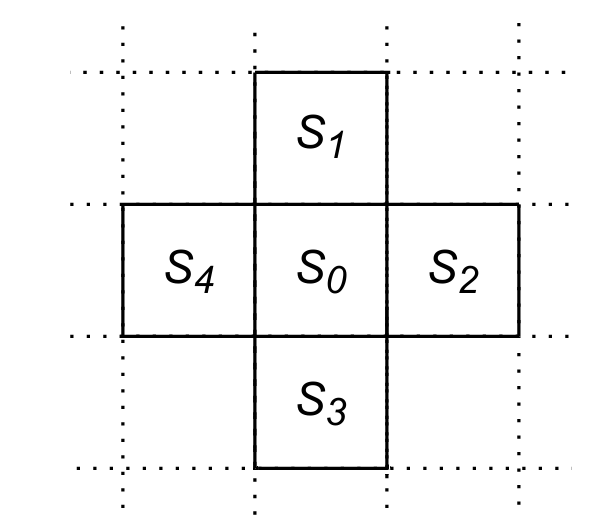
\includegraphics[scale=0.2]{pics/pics4report/full_lattice.png}
\caption{ Illustration of $S_0$ and its "nearest neighbours".}
\label{fig:spin_neighbours}
\end{figure}

This gives a flip of spin $s_0$ results in a n
energy-difference of the lattice which is
 -2 times the energy of $s_0$.
\begin{gather}
\Delta E = -2s_0(s_1 + s_2 + s_3 + s_4)
\end{gather}
It is also clear that this is quantized, which means that the 
exponential function in \eqref{eq:transition} can be precomputed.


This can be summarized in the following algorithm:
\begin{algorithm}
\begin{enumerate}[label=\arabic*)]
\item Choose start configuration. Common choices of the Ising model 
are random ($T= \infty$) and ordered ($T= 0$). 
\item Pick a random particle, $s_0$ by drawing two random integers,
$x$ and $y$ in the lattice domain.
\item Suggest a spin-flip and compute possible change in 
energy $\Delta E$.
\begin{align*} 
\Delta E = -2s_0(s_1+s_2+s_3+s_4), \quad \Delta E \in \{-8,-4,0,4,8 \} 
\end{align*} 
\item \textsc{If} $\Delta E \leq 0 \quad \to$ Accept spin-flip. \\
\textsc{Else} Draw random number, $r \in [0,1]$ \\
\textsc{	If} $r \leq exp(-\Delta E \beta ) \quad \to$ Accept spin-flip. \\
\textsc{Else} $\quad \to$ Reject flip. 

\item Repeat step 2) - 4) long enough for the system to be 
uncorrelated.

\item Collect data of interest. 

\item Repeat step 2) - 6). 
\end{enumerate}
\end{algorithm}

\subsubsection{Choice of random number generator}
The pseudo random number generator used for the simulations in 
this report is the Mersenne Twister engine
instantiated with the parameters of 
\emph{Mersenne Twister 19937 generator} seeded with the time.
This is available in the \texttt{<random>} header of the standard
library in C++ and has a period of the \emph{Mersenne number},
$2^{(n-1)w}-1$.
The instantiation chosen gives $w=32$ and $n=624$, and a period which is 
far larger than the minimum requirement.

\subsection{Computing thermodynamic properties}
The different thermodynamic properties of interest were computed 
according to the formulas \eqref{eq:Esum}, \eqref{eq:Msum} and

Specific heat:
\begin{equation}
c_v = \frac{\beta^2}{L^2}\left(\expval{E^2} - \expval{E}^2\right)
\end{equation}

Magnetic susceptibility:
\begin{equation}
\chi = \beta^2 L^2 \left(\expval{\magM^2} - \expval{\magM}^2\right)
\end{equation}

All these quantities were computed per particle and divided by the number 
of samplings.

\subsection{Finite size scaling}
\textcolor{red}{KSK:Newman and Barkema has a good section on this topic. I will write about this asap.} 

\subsection{Test environment}

The testing framework is \href{https://github.com/philsquared/Catch}{Catch}.
The test cases should be self-explanatory.


\section{Results}

\subsection{Numerical vs. analytical results for 2x2-case}

\subsection{Equilibration}
In this section we will look into how many Monte Carlo cycles are needed 
to reach the most likely state. This will be done by looking at a 
$20 \cross 20$-lattice for different dimensionless temperatures 
$\tilde{T}=1/\beta$, for both a ordered start configuration ("cold start") 
and a random start configuration ("hot start"). 
This will be done by an "by the eye"-approach, simply plotting the 
magnetisation and energy as a function of monte carlo cycles and see 
when they have only small fluctuations around some mean value. This will 
become later become out starting point for gathering data. The unstable 
phase before equilibrium is called \emph{thermalisation}.

We will also study the total number of accepted spin-flips as function of 
Monte Carlo cycles.

\subsubsection{Cold start and hot start}

\begin{figure}
\centering
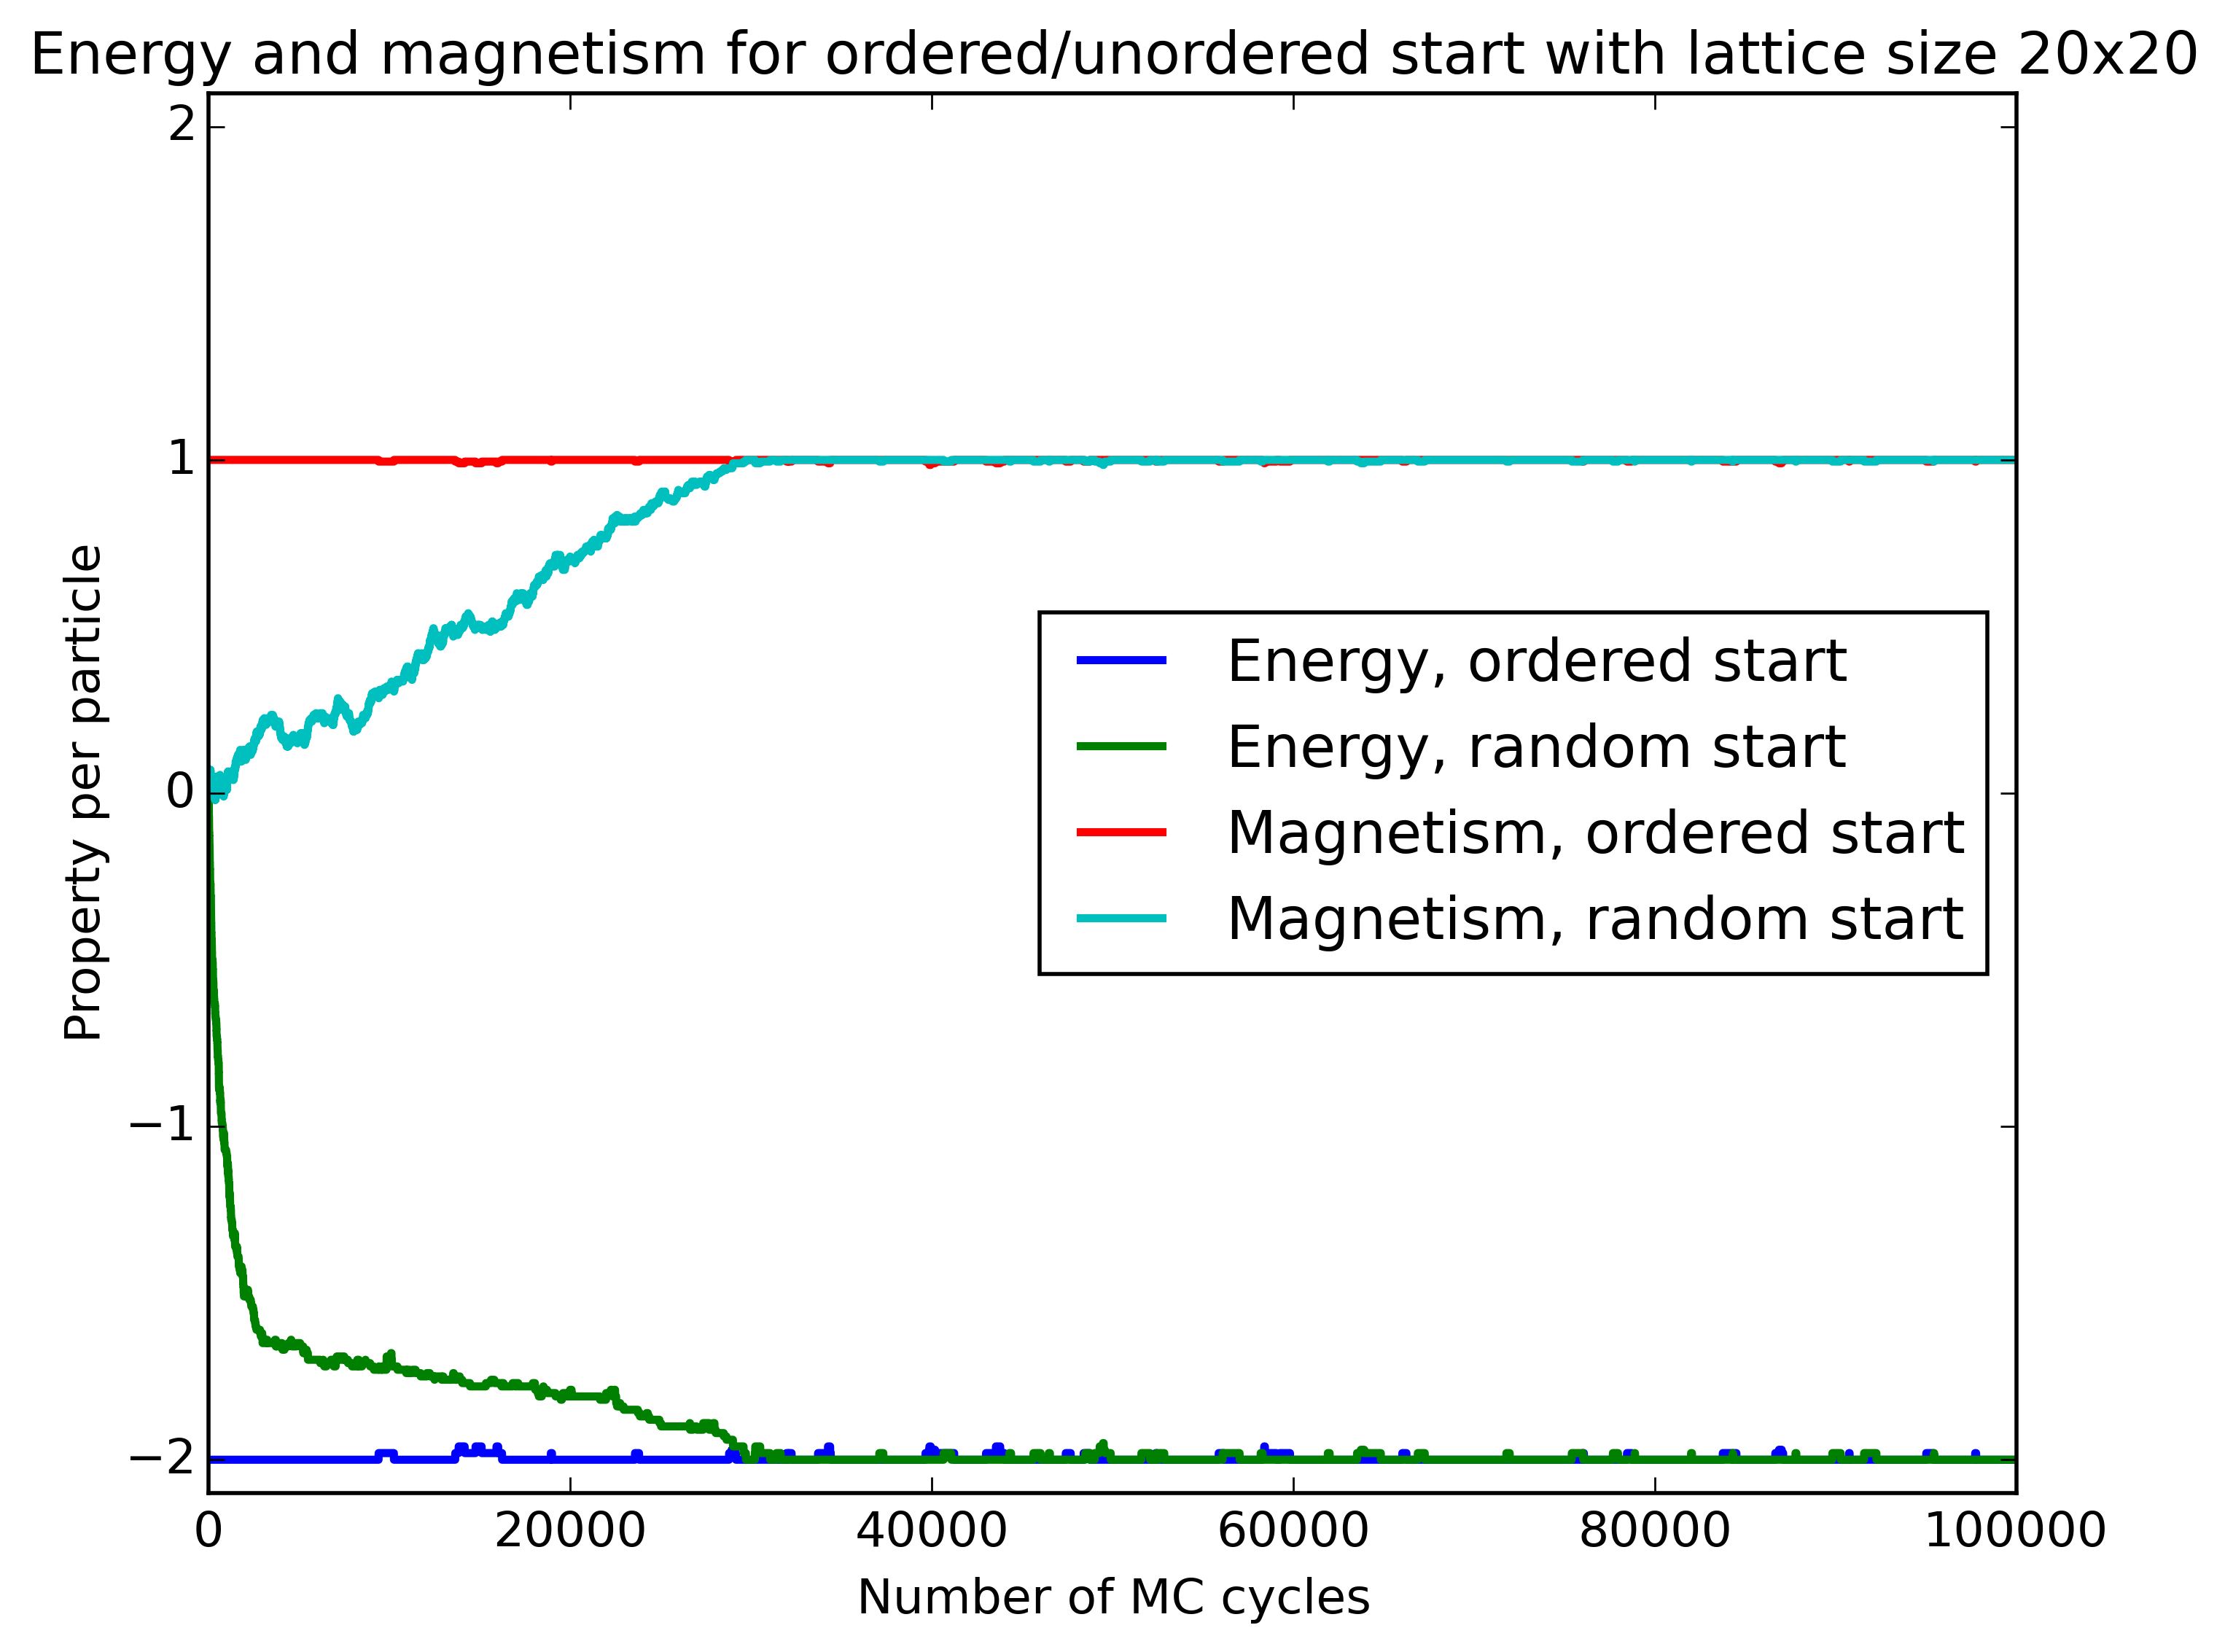
\includegraphics[width=\figurewidth]{pics/pics4report/cEM1.png}
\caption{Energy and magnetisation as a function of Monte Carlo cycles
for $\tilde{T}$ = 1}
\label{fig:EM_low_T}
\end{figure}

\begin{figure}
\centering
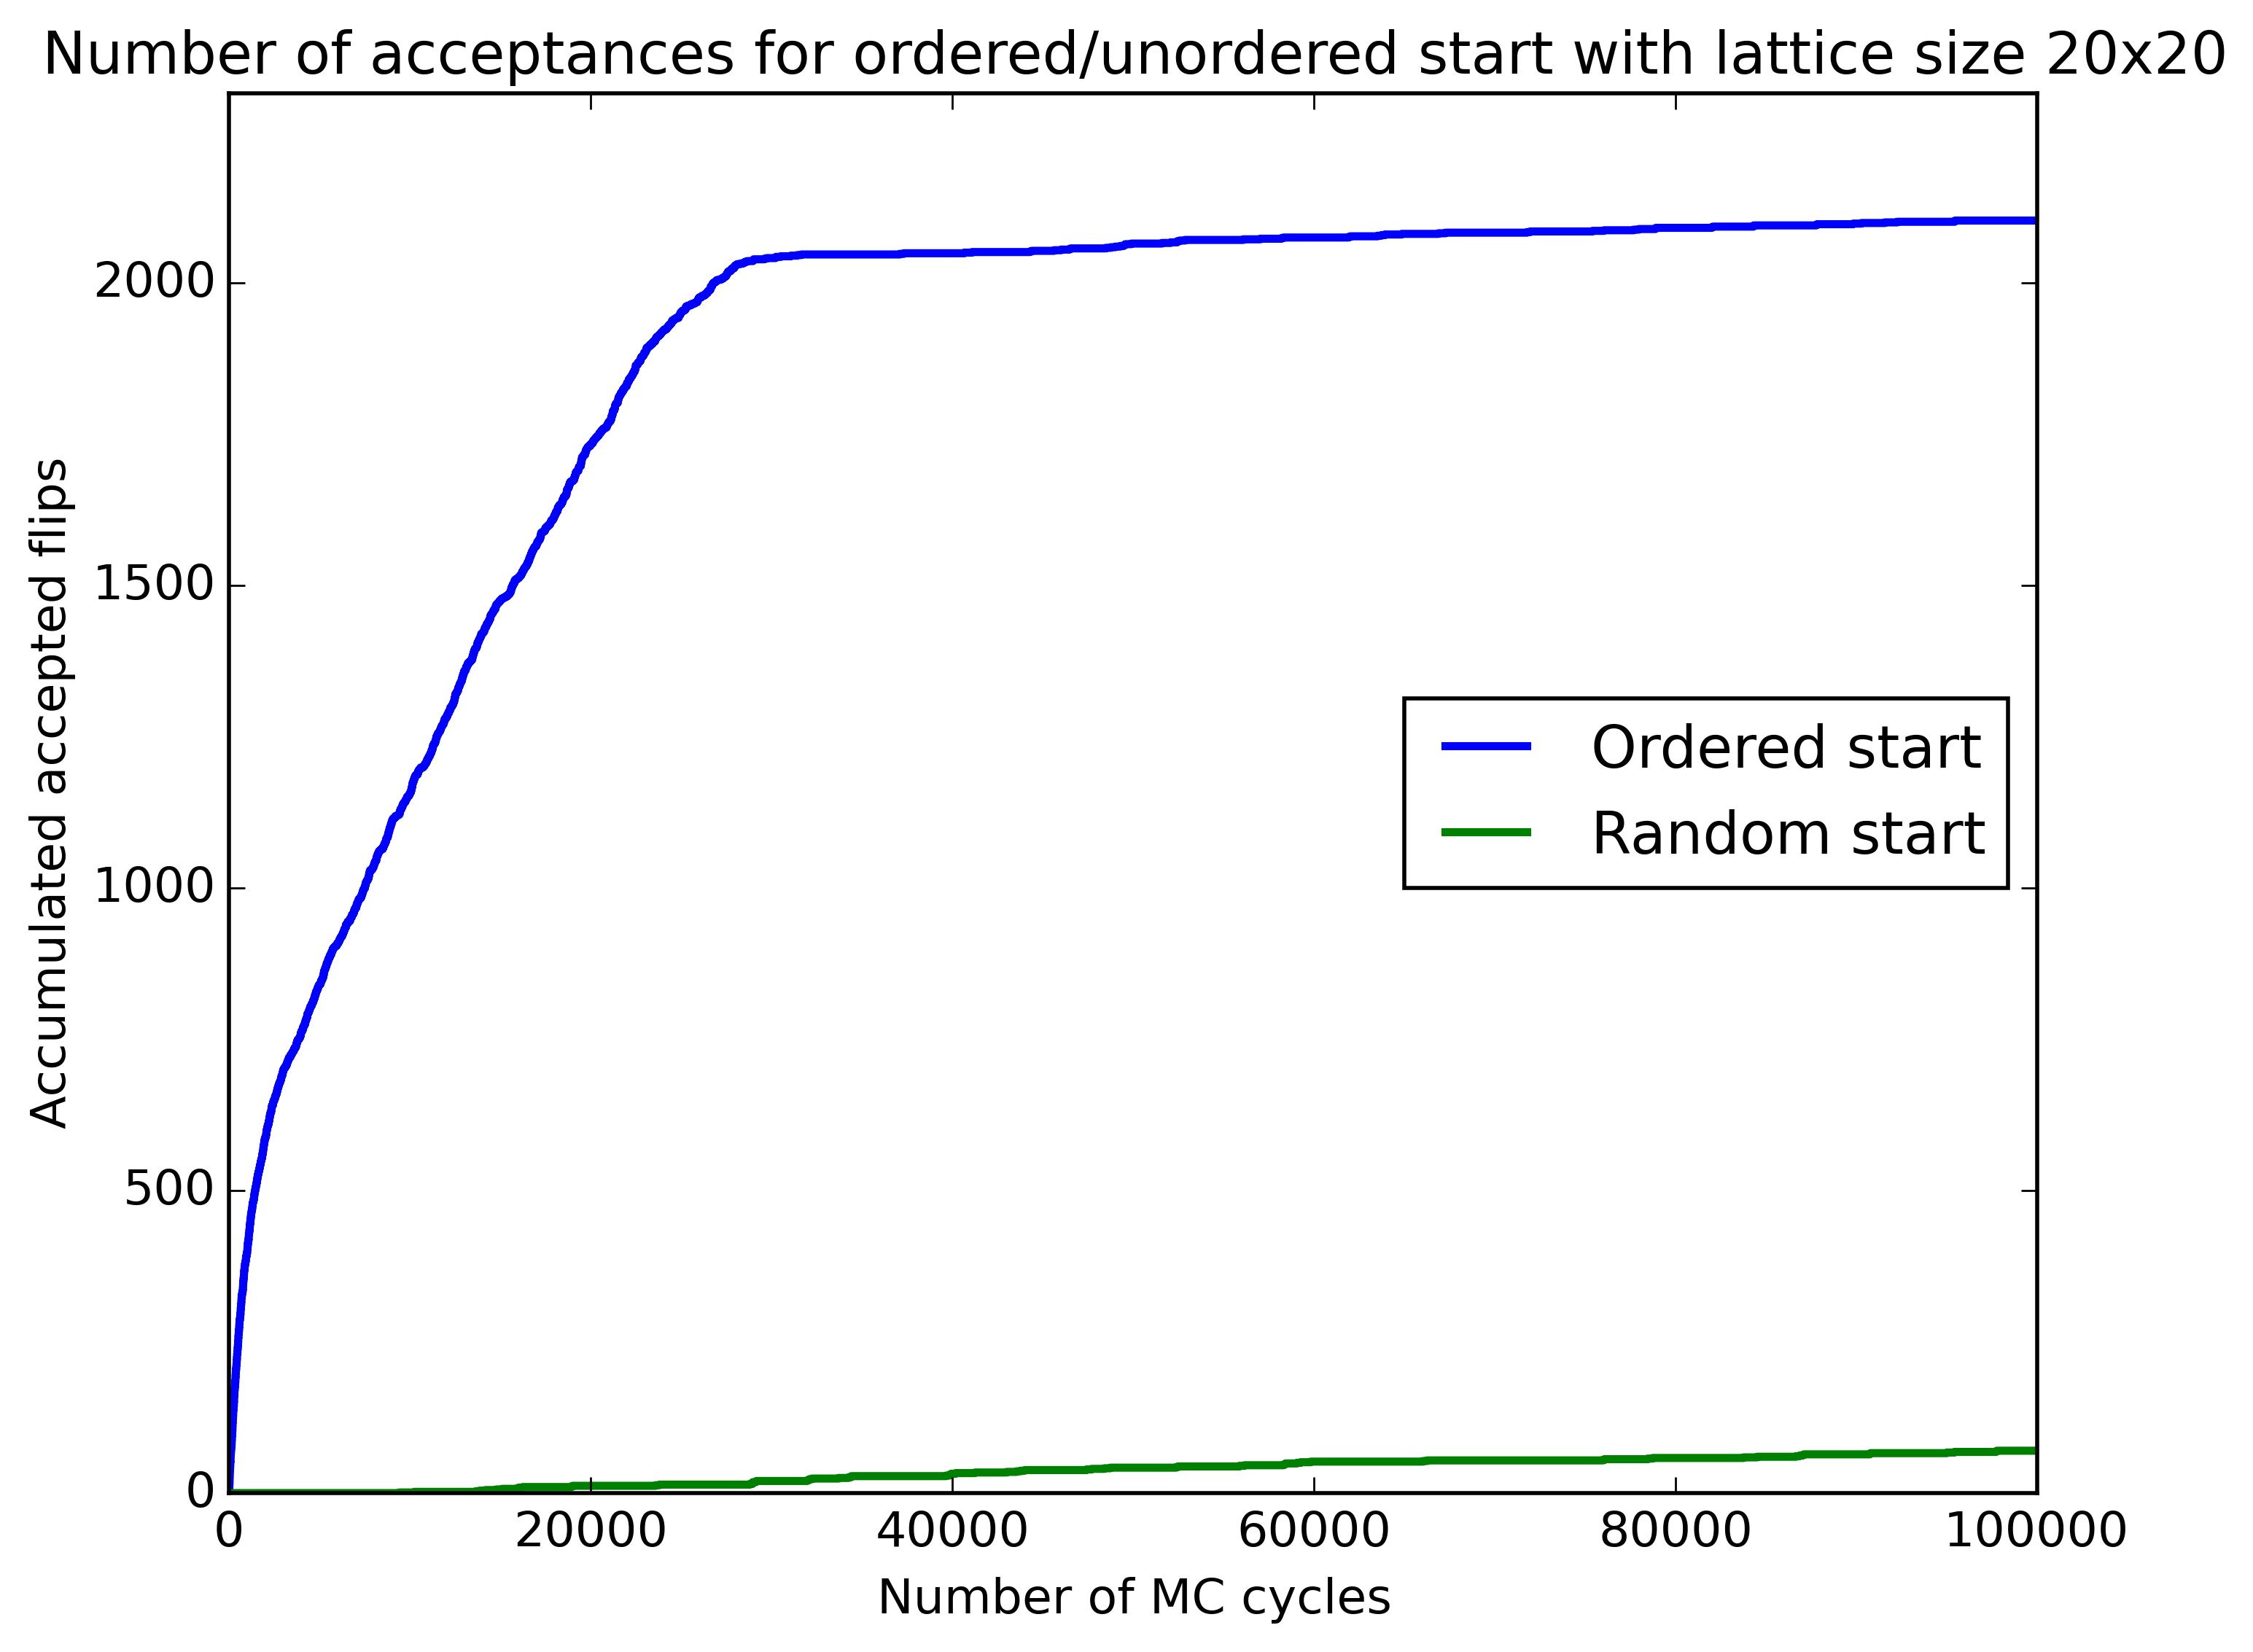
\includegraphics[width=\figurewidth]{pics/pics4report/cA1.png}
\caption{Acumulated acceptance 
for $\tilde{T}$= 1}
\label{fig:ca_low_T}
\end{figure}

\begin{figure}
\centering
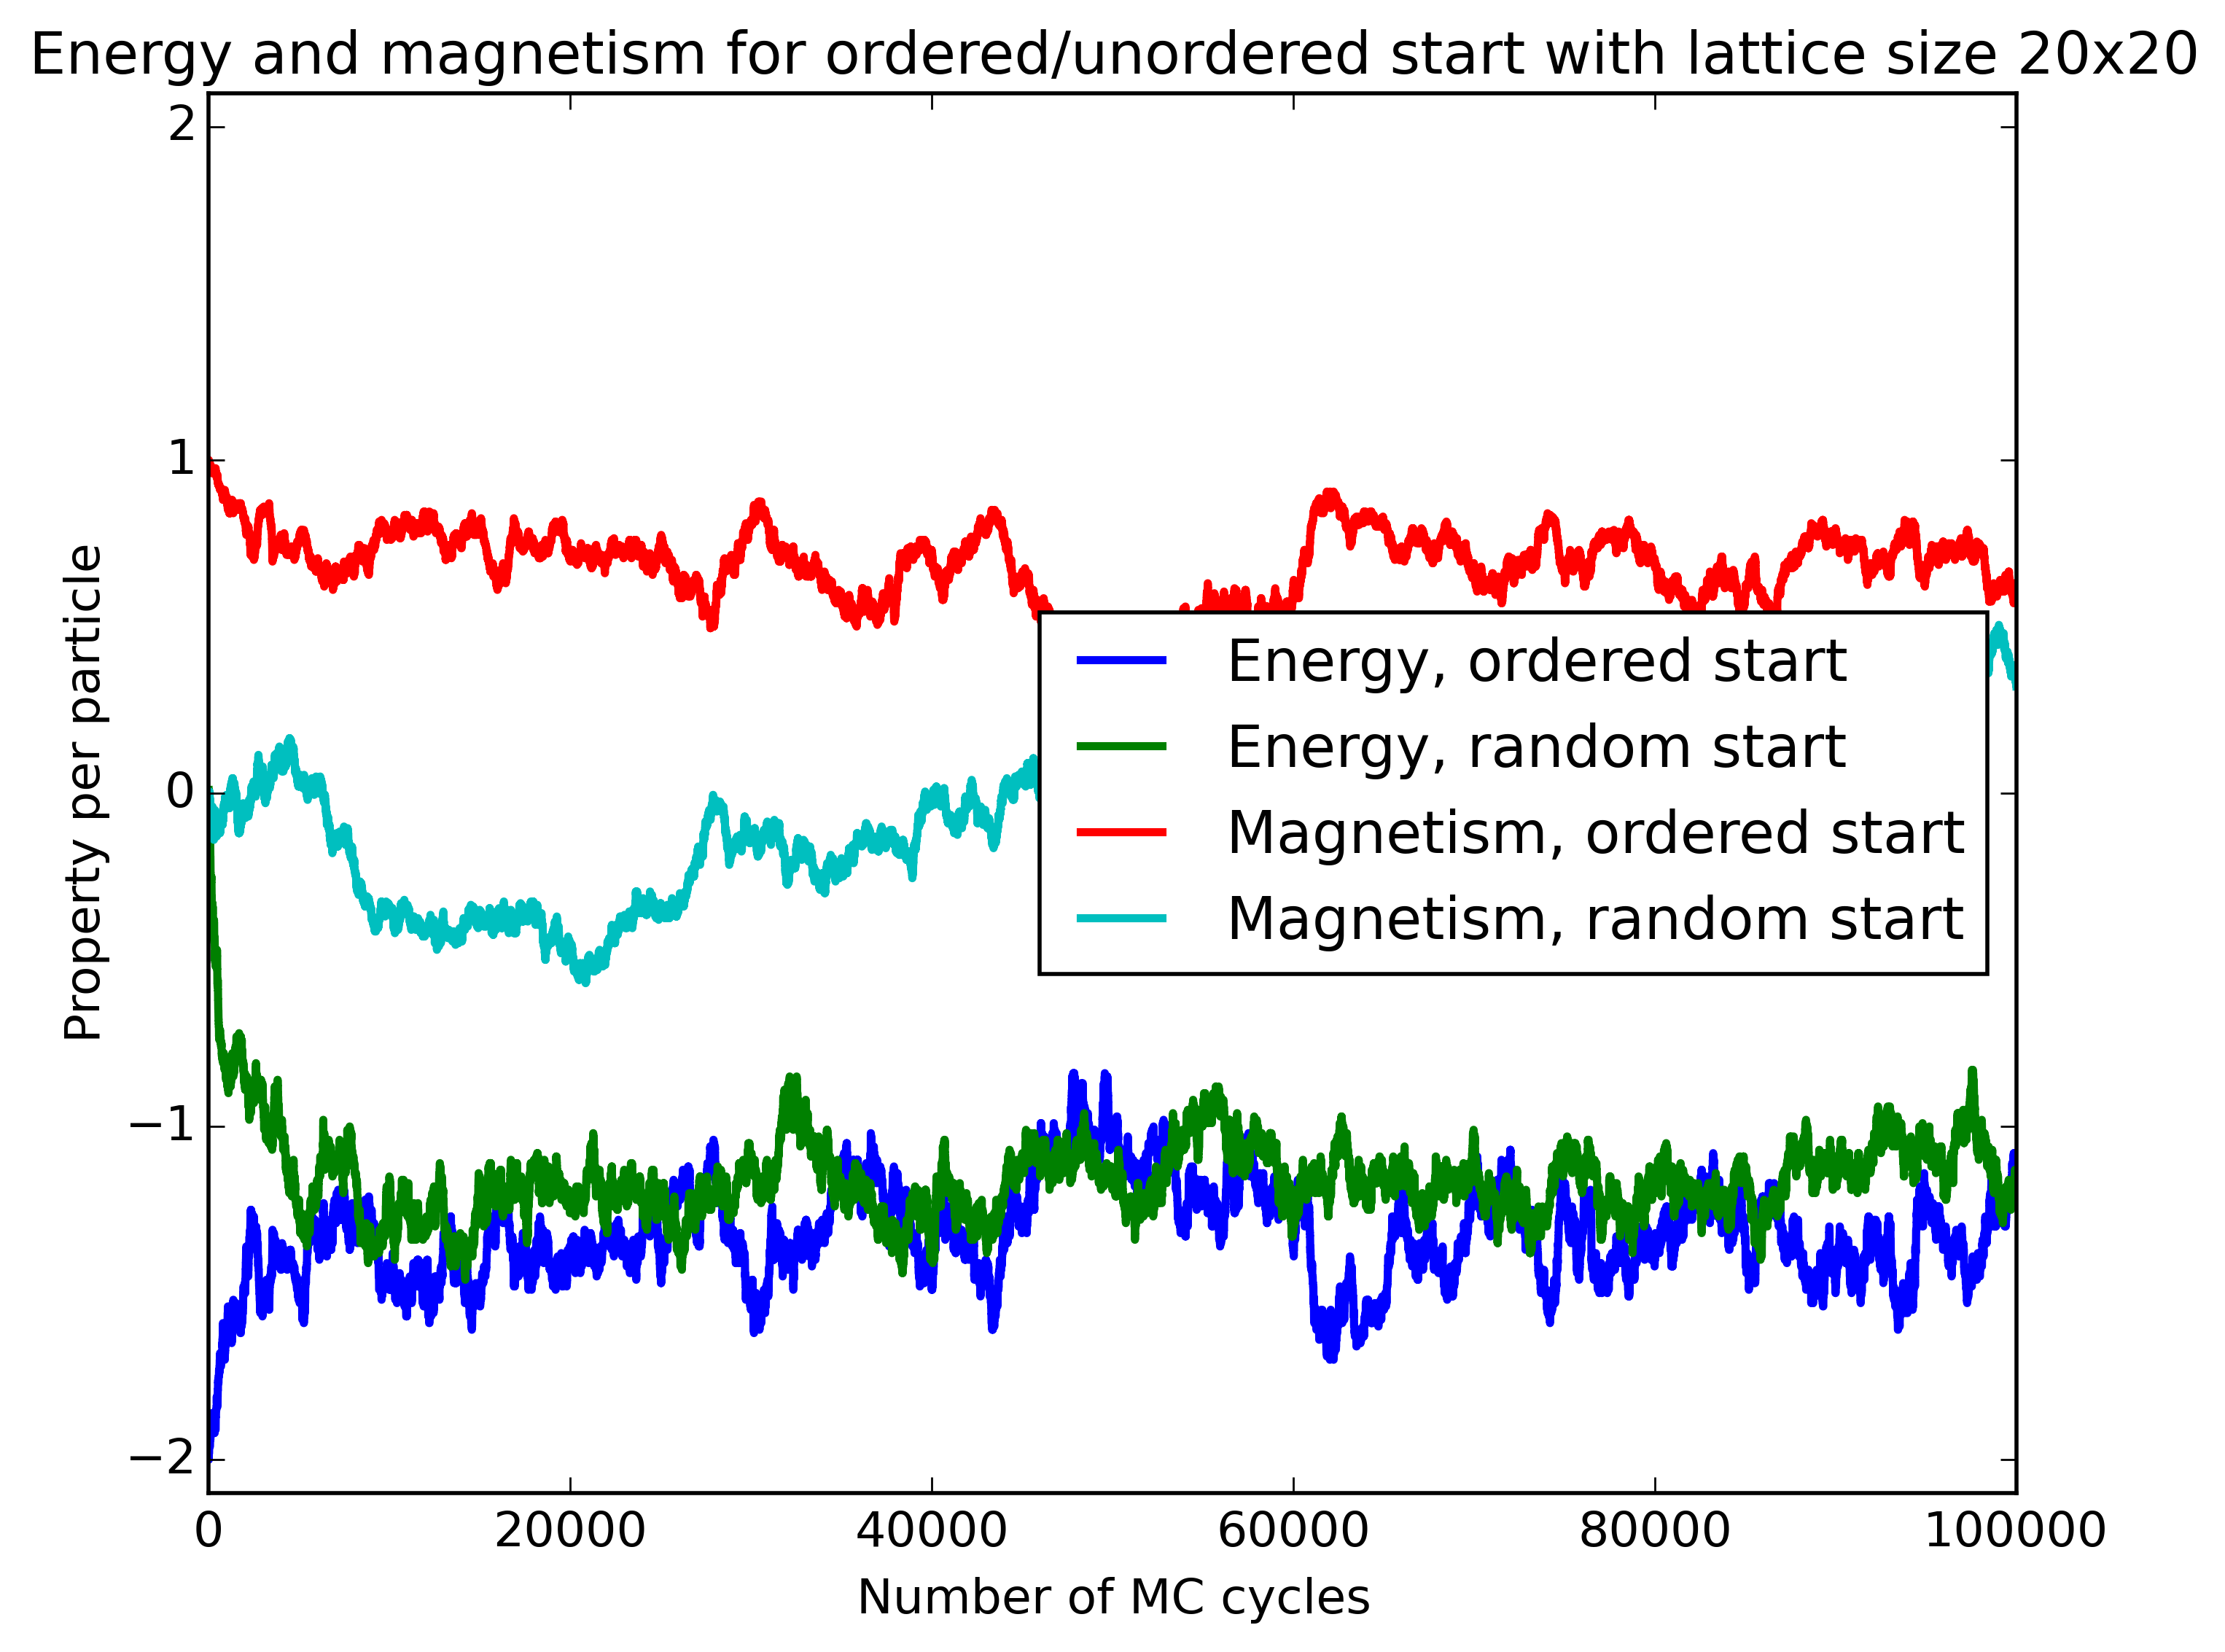
\includegraphics[width=\figurewidth]{{pics/pics4report/cEM2.4}.png}
\caption{Energy and magnetisation as a function of Monte Carlo cycles
for $\tilde{T}$= 2.4}
\label{fig:EM_high_T}
\end{figure}

\begin{figure}
\centering
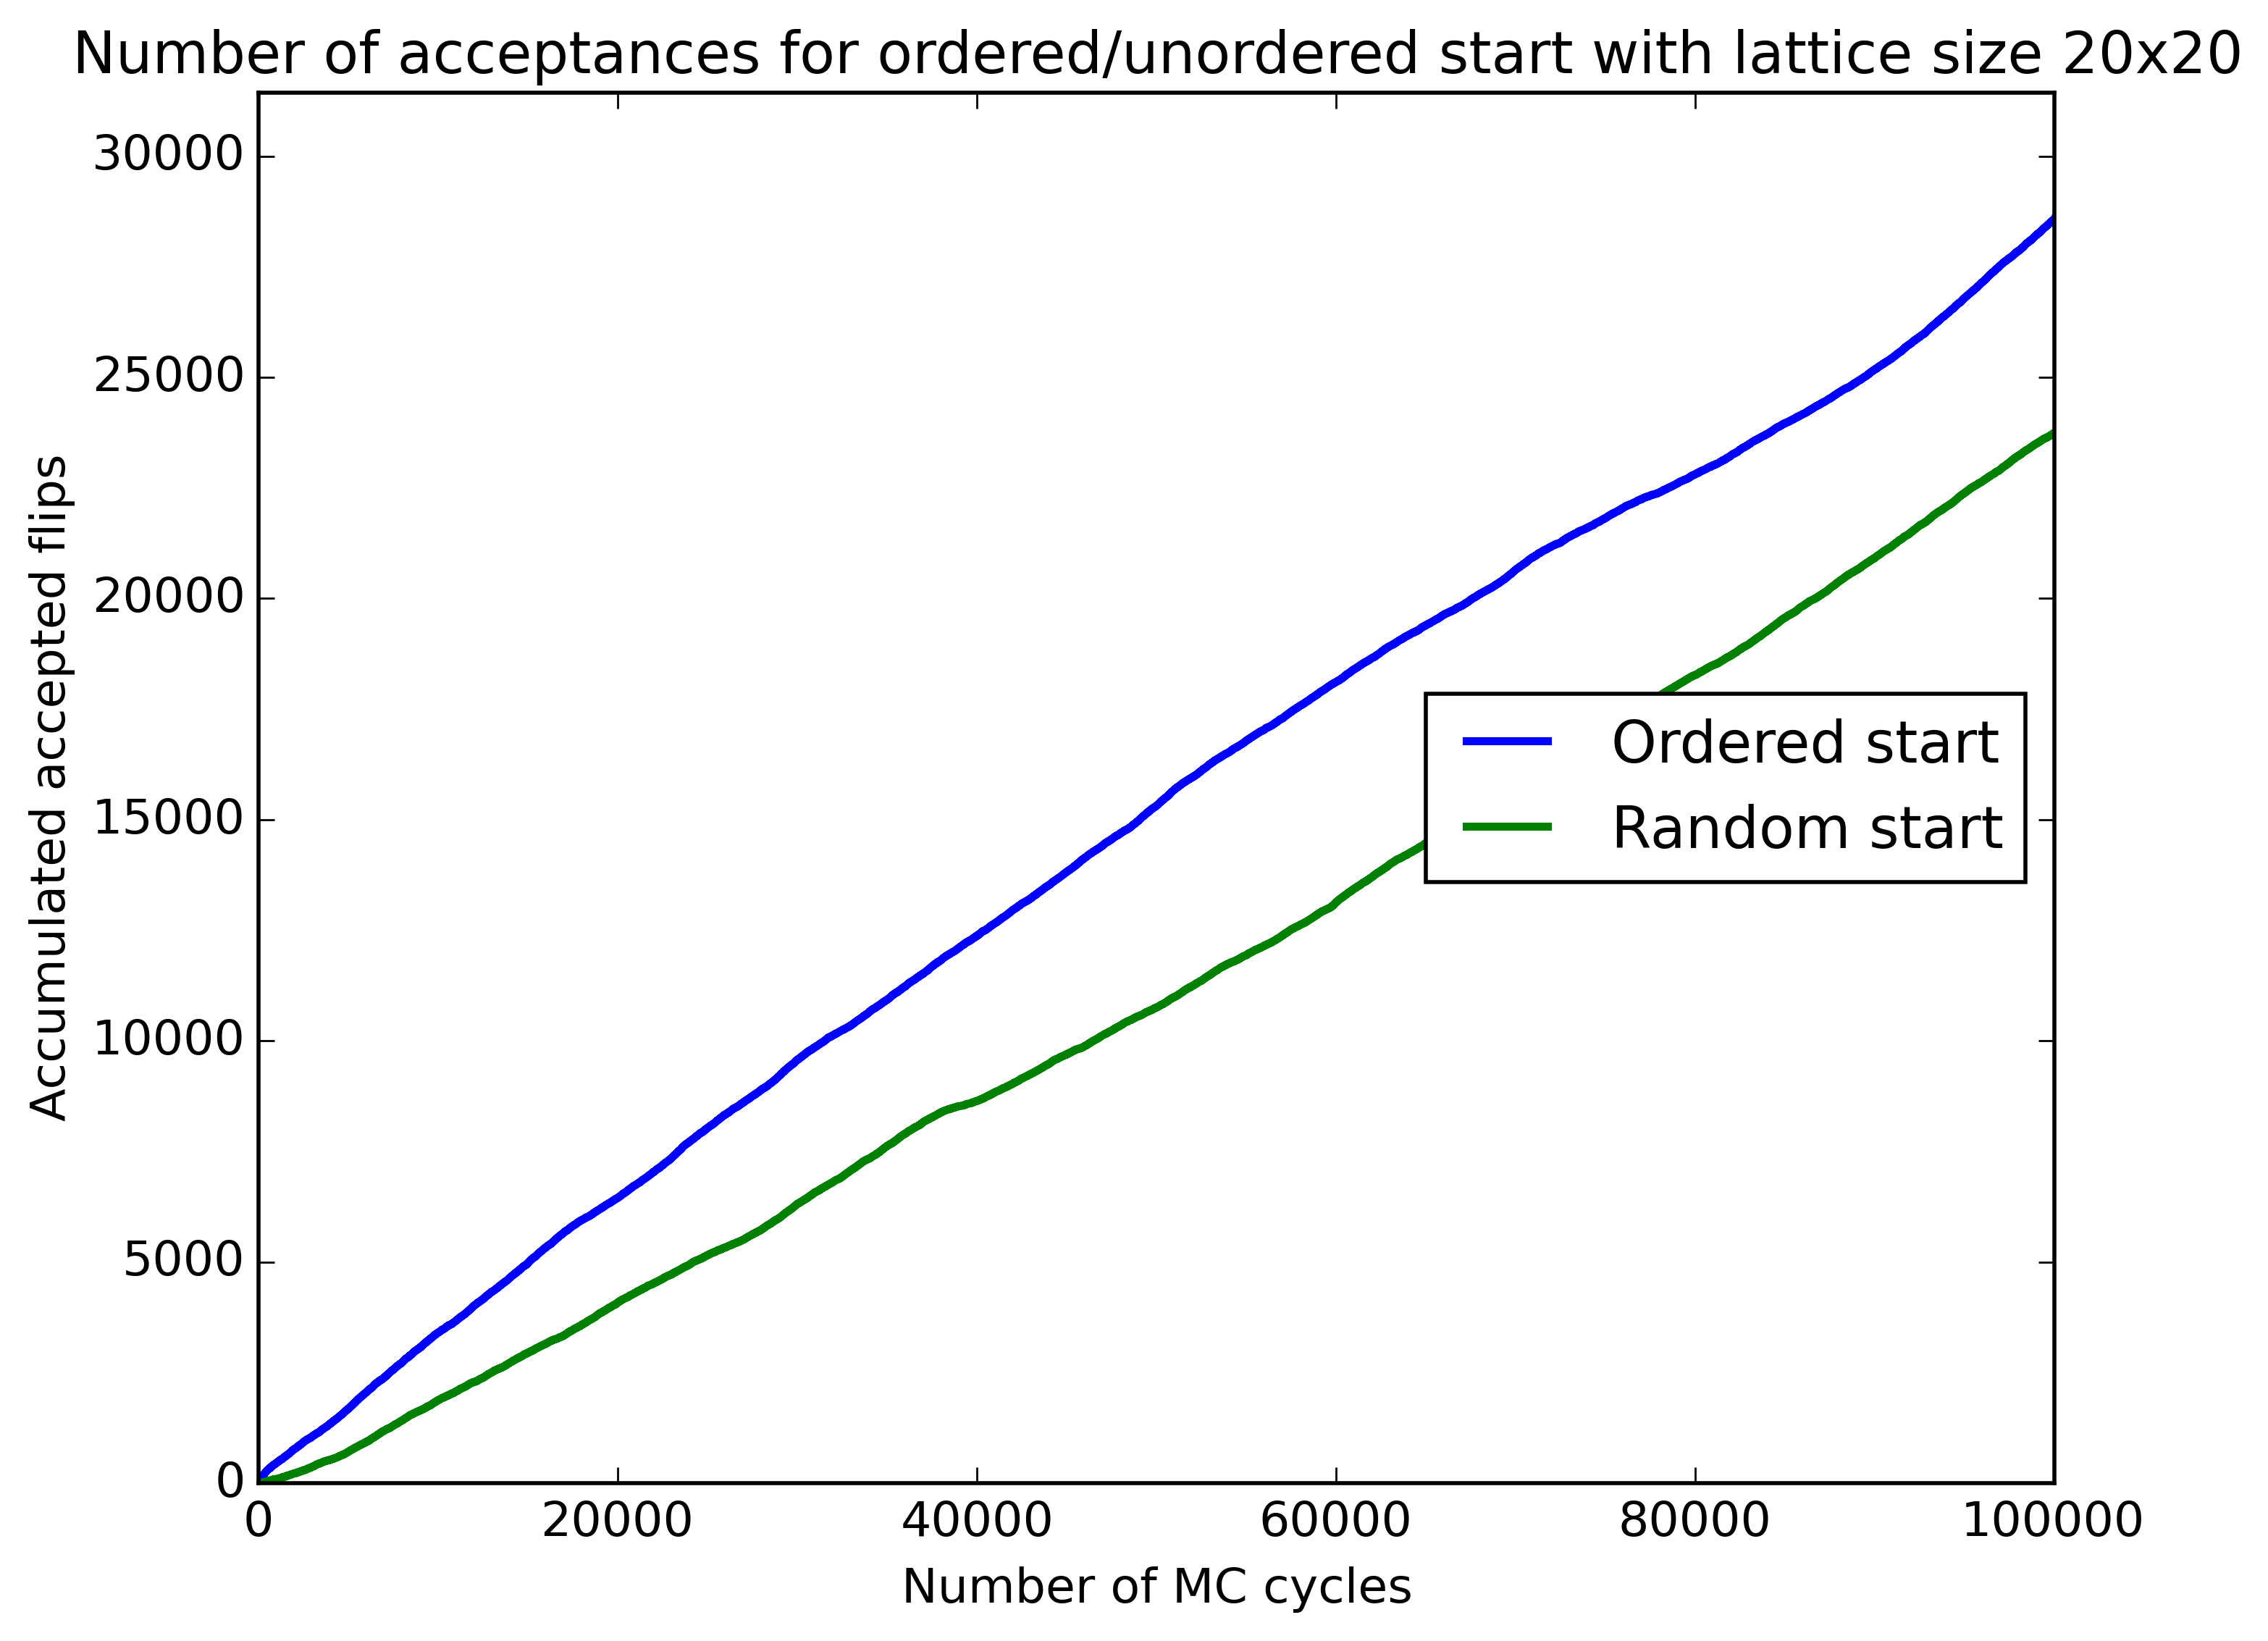
\includegraphics[width=\figurewidth]{{pics/pics4report/cA2.4}.png}
\caption{Acumulated acceptance 
for $\tilde{T}$= 2.4}
\label{fig:ca_high_T}
\end{figure}



\begin{figure}[H]
\centering
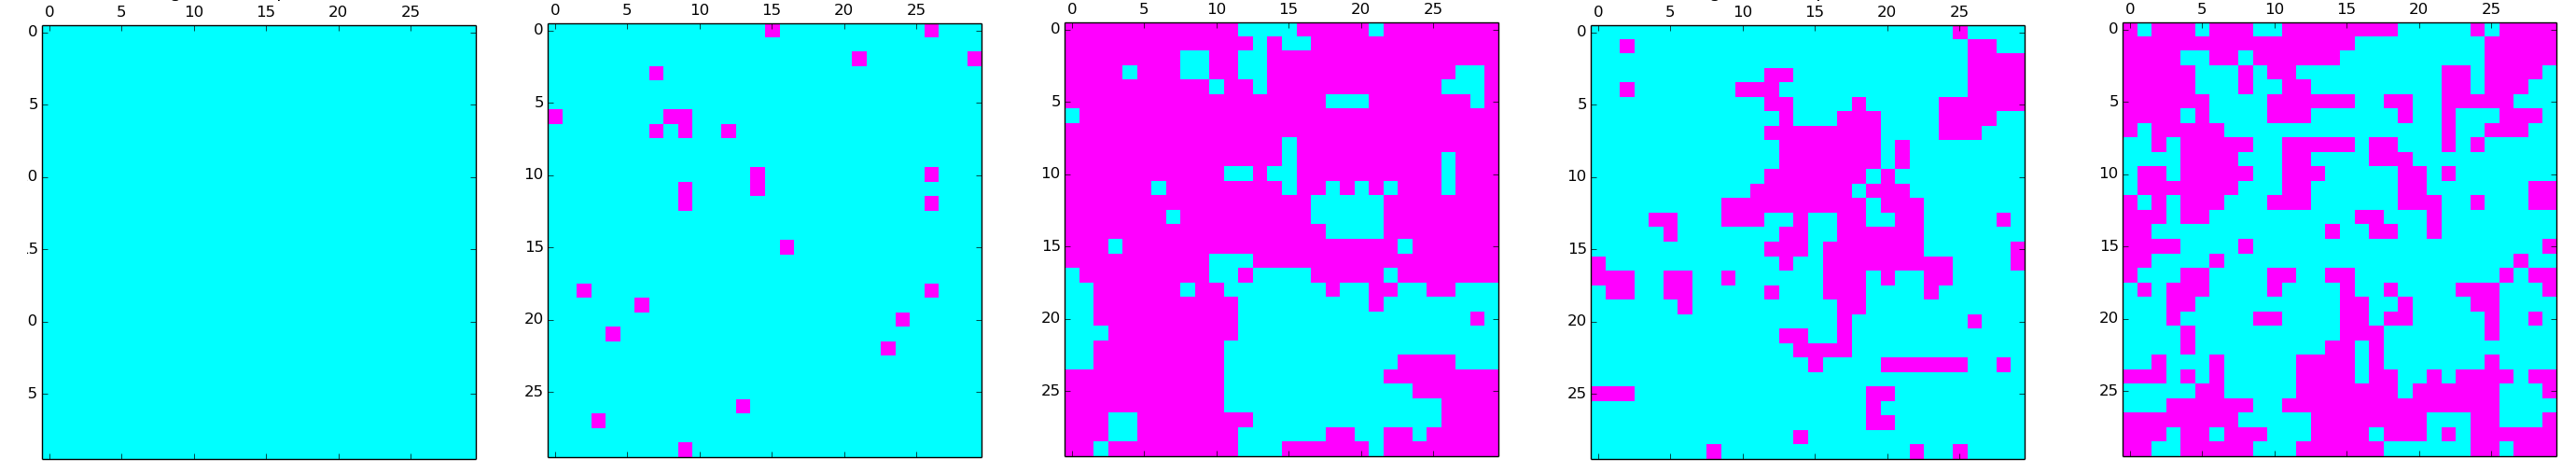
\includegraphics[scale=0.10]{pics/pics4report/equilibrium_different_temperatures.png}
\caption{Equilibrium configuration for different 
temperatures, $\tilde{T}$. Here a $30 \times 30$ lattice for 
$\tilde{T} \in\{1.0, 2.0, 2.2, 2.3, 3.0\}$. One can see the behaviour of 
the system change close to the critical temperature where the phase 
transition happens. After the phase transition all magnetization is gone.} 
\label{fig:equilibrium_T}
\end{figure}

\subsection{Computing the thermodynamic properties}

The probabilities of the different energies are in figure 
\ref{fig:dT1} and \ref{fig:dT2.4}.

\begin{figure}
\centering
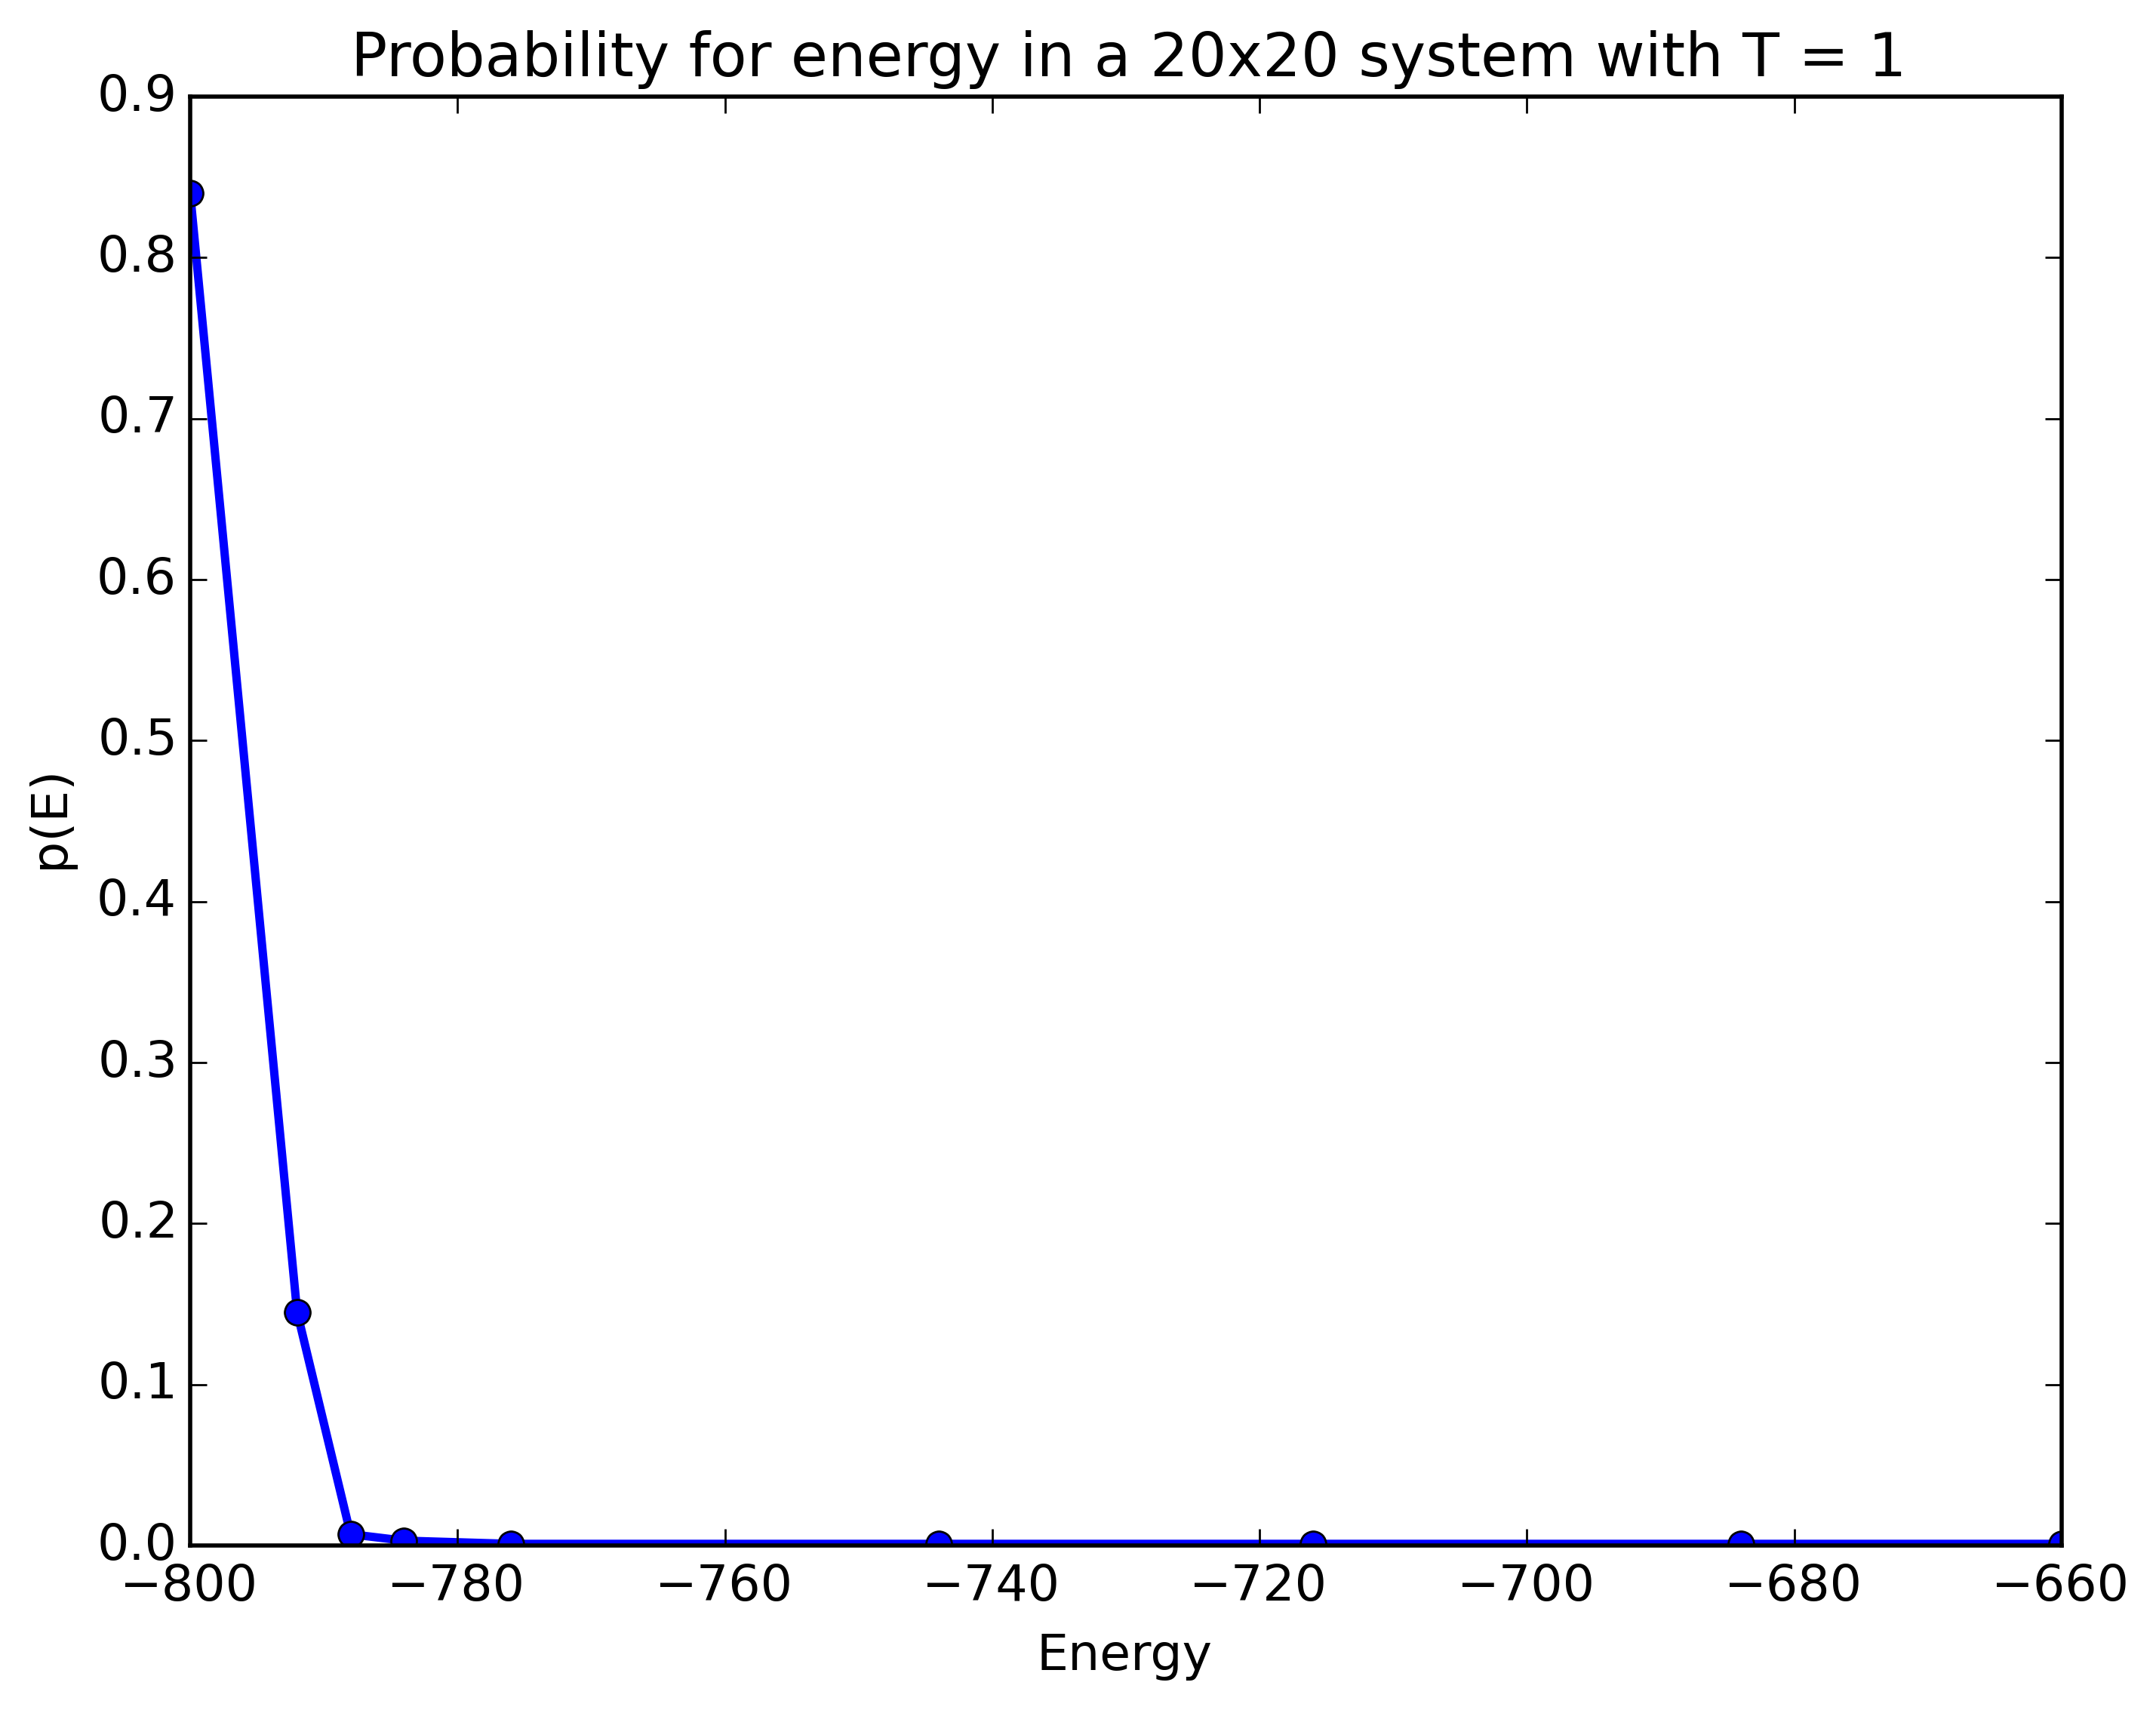
\includegraphics[width=\figurewidth]{pics/pics4report/dT=1.png}
\caption{Probabilities for the different energies for $\tilde{T}$ = 1}
\label{fig:dT1}
\end{figure}

\begin{figure}
\centering
\includegraphics[width=\figurewidth]{pics/pics4report/{dT=2.4}.png}
\caption{Probabilities for the different energies for $\tilde{T}$ = 2.4}
\label{fig:dT2.4}
\end{figure}

The properties for the different 


\subsection{Reproduction of results}

Benchmark calculations along with the programs used are available at

\url{https://github.com/mulimoen/FYS3150CompPhy/}

under the folder \emph{Project 4}.

\section{Conclusion}

\section{References}
Huang, K. 1987, \emph{Statistical mechanics}, Wiley, New York. 

Plischke, M. and Bergersen, B. 1994, \emph{Equilibrium statistical physics}, World Scientific Pub. Co., Singapore.



\end{document}